\documentclass[border=10pt]{standalone}
\usepackage{tikz}

\begin{document}
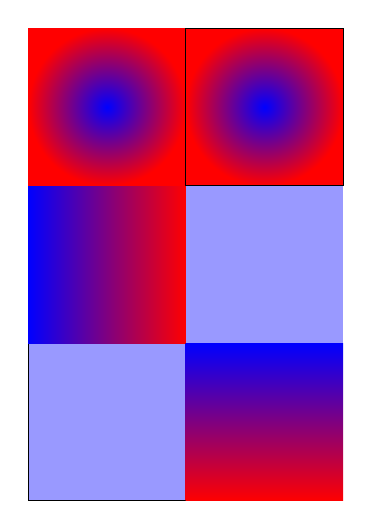
\begin{tikzpicture}[x=2cm,y=2cm] % custom unit vector lengths
\fill[blue!40!white] (1,1) rectangle (2,2);
\filldraw[fill=blue!40!white, draw=black] (0,0) rectangle (1,1); %\border
\shade[left color=blue,right color=red] (0,1) rectangle (1,2); % gradient
\shade[top color=blue,bottom color=red] (1,0) rectangle (2,1);

\shade[inner color=blue,outer color=red] (0,2) rectangle (1,3);
\shadedraw[inner color=blue,outer color=red, draw=black] (1,2) rectangle (2,3);
\end{tikzpicture}
\end{document}